\documentclass[../main.tex]{subfiles}
\begin{document}

Throughout this section, $E$ will denote $\bR^n$ equipped with the standard inner product, our fixed \textit{euclidean space}.

\subsection{Affine reflections}

This subsection roughly follows \cite{Berger2009}. When considering reflections in $E$, we don't want to just consider those lying in $O(E)$, we are also interested in reflections across some hyperplane not lying throught the origin. To tackle this we first define some standard preliminaries:

\begin{definition}
    A \textbf{reflection} in $E$ is a linear transformation $s\in O(E)$ (the orthogonal group of inner product preserving linear maps) with eigenvalues $\{-1,1\}$ with corresponding dimensions of eigenspaces:\[
        \dim{E_1} = n-1 \qquad \dim{E_{-1}} = 1
    \]
    for linear maps in $O(E)$ this is equivalent to fixing some hyperplane (codimension $1$ subspace) and having determinant $-1$.
\end{definition}

\begin{definition}
    The \textbf{group of general affine transformations} of $E$ is semidirect product of $GL(E)$ acting on $E$\[
    GA(E) := E \rtimes GL(E)
    \] where $E$ acts on itself by translation. $(v,T)\in GA(E)$ acts on $e\in E$ as $(v,T)\cdot e = v + T(e)$.
\end{definition}

\begin{proposition}
    This is actually an action. Furthermore, the action is transitive.
    \begin{proof}
        Take $(v,T), (u,S)\in GA(E)$ and $e\in E$. Showing this is an action is a direct calculation: \[
        (v,T) \cdot \pr{(u,S) \cdot e} = (v,T)\cdot \pr{u + S(e)} = v + T(u) + TS(e) = (v+T(u),TS)\cdot e = \pr{(v,T)(u,S)}\cdot e\]
        from the definition of the semidirect product. Suppose $(v,T)$ and $(u,S)$ act the same on $E$: as both $T$ and $S$ are linear the two affine transformations send $0$ to $v$ and $u$ respective, thus we have $v=u$; subtracting these equal translations and having equality means the two linear transformations must also be equal.
    \end{proof}
\end{proposition}

We can now consider appropriate affine versions of linear groups, the most important for us will be the \textbf{affine orthogonal group} $AO(E)$, which can be equivalently viewed as the subgroup of $GA(E)$ consisting of isometries, or as $E\rtimes O(E)$. We need stricter criteria than just the linear component of our affine transformation be a reflection to suitably capture the notion of a reflection across an affine hyperplane.

\begin{proposition}
    For a unit normal vector $\alpha$ and some $k\in \bR$, reflection across the affine hyperplane $(E,\alpha) = k$ corresponds to the affine transformation $(2k\alpha,s_\alpha)$, where $s_\alpha$ is the reflection along $\alpha$.\begin{proof}
        Call the affine hyperplane $H$ and choose a $v\in E$. The vector orthogonal to $H$ that goes to $v$ has length $k-(v,\alpha)$ so reflecting across $H$ send $v$ to $v+2(k-(v,\alpha))\alpha = 2k\alpha + (v-2(v,\alpha)\alpha) = (2k\alpha, s_\alpha)\cdot v$.
    \end{proof}
\end{proposition}

We call such affine transformations, \textbf{affine reflections}.

\begin{lemma}
    For all affine hyperplanes $H$ and affine reflections $r$, the set $rH$ is also an affine hyperplane.
    \begin{proof}
        Let $H$ be $\{v\in V \mid (v,\alpha)=k\}$ for some $\alpha\in E, k\in\bR$. As $r$ is bijective the set $rH$ is equal to $\{w\in V \mid (r^{-1}w,\alpha) = k\}$, by writing $r=(u,T)\in GA(E)$ this can be rewritten as $\{w\in V\mid (w,T^*(\alpha))=k-(u,\alpha)\}$, an affine hyperplane.
    \end{proof}
\end{lemma}

\begin{lemma}
    An affine transformations $r=(u,T)$ that fixes some affine hyperplane and is an involution must be an affine reflection.
    \begin{proof}
        As $r^2=\text{id}$, on $0$ we have $r^2(0)=u+T(u)=0$. So as $r^2=u+T(u)+A^2$ this means $A$ is also an involution so we can use the primary decomposition $E=E_1\oplus E_{-1}$ into the eigenspaces of $A$. Call the hyperplane $r$ fixes $H$, then for any $h=v_1+v_{-1}\in H$ (where $v_1,v_{-1}\in V_1,V_{-1}$ respectively) we have $r(v_1+v_{-1}) = u + T(v_1+v_{-1}) = u + v_1 - v_{-1} = v_1 + v_{-1}$ therefore $2v_{-1}=u$ so $\dim E_{-1}=1$ and $T$ is the reflection along $V_{-1}=\abr{v_{-1}}$, thus $r=\pr{2v_{-1},s_{v_{-1}}}$.
    \end{proof}
\end{lemma}

\begin{proposition}
    For all affine reflections $r,s$ with $s$ reflecting across the affine hyperplane $H$, the affine transformation $rsr^{-1}$ is an affine reflection across $rH$.
    \begin{proof}
        First, notice $\pr{rsr^{-1}}^2 = \text{id}$ as both $r$ and $s$ are involutions. Also, $rsr^{-1}(rH) = rH$ as $s$ fixes $H$.
    \end{proof}
\end{proposition}

From now on, we will use the umbrella term \textit{reflection} to refer to both linear and affine reflecitons.

\subsection{Reflection groups}

We are interested in groups generated by reflections in $E$, so throughout the next two sections fix a group $W\leq GA(E)$ which can be generated by reflections. This roughly follows \cite{Humphreys1990}

We would like to consider the set of all hyperplanes $H$ such that there is some affine reflection $w\in W$ across $H$ this set will be referred to as $\cH$. For certain choices of generators for $W$ we may find $\cH$ is dense in $E$.

\begin{example}
    Consider the set of hyperplanes pictured in red: 
    \begin{figure}[H]
      \centering
      \begin{subfigure}{0.45\textwidth}
        \centering
        \begin{tikzpicture}[scale=2]
          \clip (-1,-1) rectangle (2,2);
          \draw[->] (-1,0) -- (2,0) node[right] {$x$};
          \draw[->] (0,-1) -- (0,2) node[above] {$y$};
    
          \def\theta{72}
          \coordinate (A) at (0,0);
          \coordinate (B) at (1,0);
          \coordinate (C) at ($(B) + ({cos(\theta)}, {sin(\theta)})$);
          \coordinate (D) at ($(C) + ({cos(2*\theta)}, {sin(2*\theta)})$);
          \coordinate (E) at ($(D) + ({cos(3*\theta)}, {sin(3*\theta)})$);
    
          \draw[red] ($(A)!-2!(B)$) -- ($(A)!+3!(B)$);
          \draw[red] ($(B)!-2!(C)$) -- ($(B)!+3!(C)$);
          \draw[red] ($(C)!-2!(D)$) -- ($(C)!+3!(D)$);
          \draw[red] ($(D)!-2!(E)$) -- ($(D)!+3!(E)$);
          \draw[red] ($(E)!-2!(A)$) -- ($(E)!+3!(A)$);
    
          \draw[very thick,red] (A) -- (B) -- (C) -- (D) -- (E) -- cycle;
        \end{tikzpicture}
        \caption{Generating hyperplanes}
    \end{subfigure}
      \hfill
      \begin{subfigure}{0.45\textwidth}
        \centering
        \begin{tikzpicture}[scale=2]
          \clip (-1,-1) rectangle (2,2);
          \draw[->] (-1,0) -- (2,0) node[right] {$x$};
          \draw[->] (0,-1) -- (0,2) node[above] {$y$};
    
          \def\theta{72}
          \coordinate (A) at (0,0);
          \coordinate (B) at (1,0);
          \coordinate (C) at ($(B) + ({cos(\theta)}, {sin(\theta)})$);
          \coordinate (D) at ($(C) + ({cos(2*\theta)}, {sin(2*\theta)})$);
          \coordinate (E) at ($(D) + ({cos(3*\theta)}, {sin(3*\theta)})$);
    
          \draw[red] ($(A)!-2!(B)$) -- ($(A)!+3!(B)$);
          \draw[red] ($(B)!-2!(C)$) -- ($(B)!+3!(C)$);
          \draw[red] ($(C)!-2!(D)$) -- ($(C)!+3!(D)$);
          \draw[red] ($(D)!-2!(E)$) -- ($(D)!+3!(E)$);
          \draw[red] ($(E)!-2!(A)$) -- ($(E)!+3!(A)$);
    
          \coordinate (ACstart) at ($(A)!-2!(C)$);
          \coordinate (ACend)   at ($(A)!+3!(C)$);
          \coordinate (BDstart) at ($(B)!-2!(D)$);
          \coordinate (BDend)   at ($(B)!+3!(D)$);
          \coordinate (CEstart) at ($(C)!-2!(E)$);
          \coordinate (CEend)   at ($(C)!+3!(E)$);
          \coordinate (DAstart) at ($(D)!-2!(A)$);
          \coordinate (DAend)   at ($(D)!+3!(A)$);
          \coordinate (EBstart) at ($(E)!-2!(B)$);
          \coordinate (EBend)   at ($(E)!+3!(B)$);
    
          \draw[blue,name path=lineAC] (ACstart) -- (ACend);
          \draw[blue,name path=lineBD] (BDstart) -- (BDend);
          \draw[blue,name path=lineCE] (CEstart) -- (CEend);
          \draw[blue,name path=lineDA] (DAstart) -- (DAend);
          \draw[blue,name path=lineEB] (EBstart) -- (EBend);
    
          \path[name intersections={of=lineAC and lineBD, by=I1}];
          \path[name intersections={of=lineBD and lineCE, by=I2}];
          \path[name intersections={of=lineCE and lineDA, by=I3}];
          \path[name intersections={of=lineDA and lineEB, by=I4}];
          \path[name intersections={of=lineEB and lineAC, by=I5}];
    
          \draw[very thick,blue] (I1) -- (I2) -- (I3) -- (I4) -- (I5) -- cycle;
    
          \draw[very thick,red] (A) -- (B) -- (C) -- (D) -- (E) -- cycle;
        \end{tikzpicture}
        \caption{Resulting hyperplanes}
      \end{subfigure}
    \end{figure}
    As we have seen in the previous proposition, $W$ acts on $\cH$ so all the reflections of these hyperplanes, show in blue, must also lie in $\cH$. This process can be repeated to find an arbitrarily small pentagon bounded by hyperplanes. By the presence of arbitrarily close parallel hyperplanes we can see $W$ will contain arbitrarily small translations and thus $\cH$ will be dense in $E$.
\end{example}

This adds technicalities and looses the discrete geometric intuition we have for reflection groups of polytopes and lattices. To remedy this we will restrict the reflection groups we consider by requiring for any compact subset $B\subset E$, the intersection $\cH\cap B$ be finite. The set of unitvectors $\alpha \in E$ such that there exists some $H\in \cH$ with $\alpha$ normal to $\cH$ will be written $\Phi$. And without loss of generality we will assume $\Phi$ spans $E$ from here onwards.

\begin{definition}
    The connected components of $E\setminus \cH$ are called the \textbf{chambers} of $W$ in $E$.
\end{definition}

\begin{proposition}
    The number of hyperplanes touching any single chamber is finite.
    \begin{proof}
        If the group is finite this is obvious. Assume the group is infinite and the chambers are not all bounded (otherwise the restriction applies directly), if there are any parallel hyperplanes thus translations then all parallelism classes of hyperplanes will be translated and as $\Phi$ is assumed to be spanning every alcove will be bounded. It turns out to be impossible to have no parallel planes, and the group to be both infinite and locally compact, see \cite{Humphreys1990} for the full proof.
    \end{proof}
\end{proposition}

We now want to choose a chamber $C_0$, and consider the set of hyperplanes $\{H_1,\ldots,H_k\}\subseteq \cH$ bounding $C$. We will call the corresponding reflections across these hyperplanes $\{s_1,\ldots,s_k\}$ \textbf{simple reflections}.

\begin{theorem}
    The set of simple reflections $\{s_1,\ldots, s_k\}$ generates $W$.
    \begin{proof}
        Let $W'$ be the subgorup of $W$ generated by the simple reflections. Let $s$ be one of the reflections generating $W$, and call the hyperplane it reflects across $H$. If $W'$ acts transitively on the set of chambers then there will exists some $w\in W'$ such that $wH_i=H$ for some simple reflection $s_i$ as $H$ will must bound a chamber. Thus, by an earlier lemma, $ws_iw^{-1} = s$ so $s\in W'$ and $W=W'$.
        Now we just have to show the action of $W'$ is transitive on chambers. Suppose it isn't, i.e. there is some chamber $C$ such that no $w\in W'$ satisfies $wC=C_0$. Let $C'$ be the closest chamber to $C_0$ in the $W'$ orbit of $C$, as $C'\neq C_0$ there must be some simple hyperplane (the boundary of $C_0$) between them, reflecting across this must strictly decrease the distance between the two chambers contradicting the minimality of $C'$. Thus $W'$ acts transitively on the set of chambers.
    \end{proof}
\end{theorem}

As a direct corollary of this proof we now know $W$ acts transitively on the set of chambers. Before discussing this further we should examine the relations that these simple reflections satisfy.

For any two simple reflections $s_i,s_j$ the subgroup $\abr{s_i,s_j}$ will be dihedral, as seen in the previous section, (note that this will be the infinite dihedral group iff the hypeplanes being reflected along are parallel), call the order of this dihedral group $2m_{ij}$. The product $s_i s_j$ will have order $m_{ij}$ in $W$ and so $W$ satisfies the set of relations $(s_is_j)^{m_{ij}}=\text{id}$ for all $i,j$, taking $m_{ii}=1$. A group \textit{presented} by these relations is called \textbf{Coxeter}.

\begin{definition}
    A \textbf{Coxeter system} is a pair $(W,S)$ where $S=\{s_i\}_{i\in I}$ is a generating set for $W$ which admits the presentation:\[
        W = \abr{S \mid (s_is_j)^{m_{ij}} \text{ for all } i,j\in I}
    \]
    where each $m_{ij}\in \bN\cup\{\infty\}$.
\end{definition}

To each Coxeter system we can assign a \textbf{Coxeter diagram}: an undirected graph created by the following rules:\begin{itemize}
    \item Draw a node $i$ for each $s_i\in S$;
    \item For each relation $(s_i s_j)^{m_{ij}}$ with $m_{ij}>2$ draw an edge between $i$ and $j$ and label it with $m_{ij}$.
\end{itemize}

This process can be reversed to obtain a Coxeter system from any Coxeter diagram. This correspondence will associate the graph:
\begin{figure}[!h]
\centering
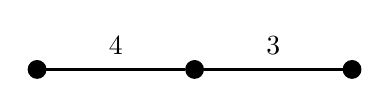
\begin{tikzpicture}
    \begin{scope}[every node/.style={circle, fill=black, draw, thick, minimum size = 6pt, inner sep=0pt}]
        \node (1) at (0,0) {};
        \node (2) at (2,0) {};
        \node (3) at (4,0) {};
    \end{scope}

    \begin{scope}[every edge/.style={draw,very thick}]
        \path [-] (1) edge (2);
        \path [-] (2) edge (3);
        \node at (1,0.3) {$4$};
        \node at (3,0.3) {$3$};
    \end{scope}
\end{tikzpicture}
\end{figure}

to the group presentation: \[
\abr{s_1,s_2,s_3 \ \middle| \ s_1^2 = s_2^2 = s_3^2 = e, \ (s_1s_2)^4 = (s_2s_3)^3 = (s_1s_3)^2 = e}
\]

In the future, for the sake of readability, the $3$ labels will often be excluded.

The classification of finite reflection groups goes by proving all reflection groups are in fact Coxeter groups and then classifying all the finite Coxeter groups.

\subsection{Coxeter presentation}

We have shown the action of $W$ on the set of chambers is transitive, but we need a stronger notion to prove these groups are Coxeter.

\begin{definition}
    Let $G$ be a group acting on a set $X$, the action is called \textbf{simply transitive} if for all $x,y\in G$ there exists a unique $g\in G$ such that $g\cdot x = y$.
\end{definition}

By fixing a base point $x\in X$ there is clear a 1-to-1 correspondence between $X$ and $G$: associate $e\leftrightarrow x$ and for all $g\in G$, $g\leftrightarrow g\cdot x$.

\begin{proposition}
    An action is simply transitive iff it is transitive and free.
    \begin{proof}
        An action is transitive if for all $x,y\in X$ there exists some $g\in G$ such that $g\cdot x = y$, and free if there exists at most one such $g$; therefore these statements are equivalent.
    \end{proof}
\end{proposition}

If we know the action is trasntive a priori we only need to check the free condition on a single element. So showing our action is simply transitive ammounts to showing for all $w\in W$ such that $wC_0 = C_0$ we have $w=\text{id}$.

We will go about prooving this by finding a geometric interpretation of the length of a word $w\in W$ in terms of simple reflections.

\begin{definition}
    For $w\in W$ define the \textbf{length} of $w$, $l(w)$ to be the minimal positive integer $r$ such that $w=s_1\cdots s_r$, a length $r$ product of simple reflections.
\end{definition}

And the contrasting way to compute the length: for any $w\in W$ consider the set of hyperplanes $H$ such that $C_0$ and $wC_0$ lie on different sides of $H$. Call this $\cL(w)$ and let $n(w) = |\cL(w)|$.

\begin{lemma}
    \begin{enumerate}
        \item $n(w) = n(w^{-1})$,
        \item $l(w) = 1$ iff $w$ is a simple reflection
        \item $l(w) = l(w^{-1})$
        \item if $w$ can be written as $s_1\cdots s_r$ then $\det(w) = (-1)^r$
        \item $l(s_i w),l(w s_i) = l(w) \pm 1$
    \end{enumerate}
    \begin{proof}
        ($1.$) $H$ separtes $C_0$ and $w^{-1}C_0$ iff $wH$ separates $wC_0$ and $C_0$ --- $W$ acts isometrically.
    \end{proof}
\end{lemma}

\begin{lemma}
    $H_i$ is in exactly one of $\cL(w)$ or $\cL(s_i w)$
\end{lemma}

\begin{lemma}
    Choose a simple hyperplane $H_i$, for any hyperplane $H\neq H_i$ and $w\in W$, if $H\in \cL(w)$ then $s_iH\in \cL(s_i w)$.
    \begin{proof}
        As $H$ separates $C_0$ and $wC_0$, $s_iH$ separates $s_i C_0$ and $s_i w C_0$, so $s_i H$ is in exactly one of $\cL(s_i)$ or $\cL(s_i w)$, but if $s_i H \in \cL(s_i)$ we would have $s_i H = H_i \implies H=H_i$ a contradiction. Therefore $s_i H \in \cL(s_i w)$.
    \end{proof}
\end{lemma}

\begin{corollary}
    $s_i\pr{\cL(w)\setminus \{H_i\}} = \cL(s_i w) \setminus \{H_i\}$.\begin{proof}
        by applying the previous lemma to both $w$ and $s_i w$ we get the required iff.
    \end{proof}
\end{corollary}

\begin{proposition}
    For all $w\in W$, we have $n(w)\leq l(w)$.
    \begin{proof}
        If $l(w) = 1$ then $w$ must be some simple reflection $s_i$ so $\cL(w) = \{H_i\}$\citationneeded so $n(w)=1$. Now by induction on $l(w)$: if $l(s_i w) = l(w) + 1$ then by the previous corollary and an earlier lemma we know $n(s_i w) = n(w) \pm 1$, namely $n(s_i w) \leq n(w) + 1 = l(w) + 1 = l(s_i w)$.
    \end{proof}
\end{proposition}

Now to show $n(w)=l(w)$ we will enumerate the hyperplanes in $\cL(w)$.

\begin{lemma}
    If $w=s_1\cdots s_r$ is a reduced expression for $w$ in terms of simple reflections, the hyperplanes:\[
        H_1, s_1 H_2, s_1s_2H_3,\ldots s_1\cdots s_{r-1} H_r
    \] are all distinct.
    \begin{proof}
        Suppose, for a contraditction, that there exists some $1\leq i < j \leq r$ such that the hyperplanes $s_1 \cdots s_{i-1} H_i$ and $s_1\cdots s_{j-1} H_j$ are equal, by applying $s_1\cdots s_{i-1}$ to both sides this implies $H_i = s_i\cdots s_{j-1}H_j$, by an earlier corollary this implies $s_i = (s_I\cdots s_{j-1})s_j(s_{j-1}\cdots s_i)$ which implies $s_{i+1}\cdots s_{j-1} = s_i\cdots s_j$ contradicting the minimality of the lenght of $w$.
    \end{proof}
\end{lemma}

\begin{proposition}
    If $w=s_1\cdots s_r$ is a reduced expression for $w$ in terms of simple reflections: \[
        \cL(w) = \{H_1, s_1 H_2, s_1s_2H_3,\ldots s_1\cdots s_{r-1} H_r\}
    \]
    \begin{proof}
        We go by induction on $r$. Observe the base case $\cL(s_1) = \{H_1\}$ from an earlier lemma. Now assume the claim holds for all $w$ with reduced length $<r$ specifically:\[
            \cL(s_1w) = \{H_2, s_2H_3,\ldots s_2\cdots s_{r-1} H_r\}
        \] we know from an earlier lemma $H_1$ is in exactly one of $\cL(w)$ or $\cL(s_1w)$. If $H_1\in \cL(s_1w)$ by applying $s_1$ we would have for some $i>1$: \[
            s_1H_1 = H_1 = s_1\cdots s_i H_i
        \] which contradicts the previous lemma, thus $H_1\in \cL(w)$, combining this with the earlier corollary gives the desired result.
    \end{proof}
\end{proposition}

A direct consequence of this propsition is that if some $w\in W$ is such that $wC_0 = C_0$ then $\cL(w)=\emptyset$ which implies $w=\text{id}$ in reduced form. We know this is sufficient to say the action of $W$ on the set of chambers is simply transitive.

We can now prove two key combinatorial properties of the reflection group, and use these to show all relations in $W$ are direct consequences of those in the Coxeter presentation.

\begin{theorem}[Exchange Condition]
    If $w\in W$ has reduced expression in terms of simple reflections $w=s_1\cdots s_r$ and $l(sw)<l(w)$ for some simple reflection $s$, there exists some $1\leq i\leq r$ such that $w = ss_1\cdots s_{i-1}s_{i+1}\cdots s_r$.
    \begin{proof}
        We know:\[
            \cL(w) = \{H_1, s_1 H_2, s_1s_2H_3,\ldots s_1\cdots s_{r-1} H_r\}
        \] by a previous proposition we know $H$, the hyperplane corresponding to $s$, must lie in $\cL(w)$ and so for some $1\leq i \leq r$, $H=s_1\cdots s_{i-1} H_i$ which implies $s=s_1\cdots s_{i-1} s_i s_{i-1}\cdots s_1$ therefore $ss_1\cdots s_{i-1} = s_1\cdots s_i$. Substituting this back into $w$ gives the desired result.
    \end{proof}
\end{theorem}

\begin{theorem}[Deletion Condition]
    If $w\in W$ has a nonreduced expression in terms of simple roots $w=s_1\cdots s_r$ then there exists $1\leq i,j \leq r$ such that $w=s_1\cdots \hat{s_i}\cdots\hat{s_j}\cdots s_r$. The hats denote omission.
    \begin{proof}
        For this to be nonreduced there must eventually exist some $i$ such that $l(s_i\cdots s_r) = l(s_{i+1}\cdots s_r) -1$ so by the exchange condition $s_{i+1}\cdots s_r = s_i s_{i+1} \cdots \hat{s_j} \cdots s_r$. Substituting this back into $w$ gives the desired result.
    \end{proof}
\end{theorem}

Note that the following result, coming initially from the geometry of the reflection group, is actually a direct consequence of the Coxeter relations and nothing more. In \ref{geom:rep} we see how we can explicitly recover this geometry from the Coxeter presentation.

\begin{theorem}
    Any finite reflection group satisfies the Coxeter presentation.
    \begin{proof}
        As in \cite{Humphreys1990} we go informally by reasoning about the smallest nontrivial relation $w=s_1\cdots s_r = \text{id}$, in terms of simple reflections, in $W$ which is not a consequence of the Coxeter relations.

        By examining the determinants, we see $r=2k$ must be even, thus we can write $s_1\cdots s_{k+1} = s_{k+2}\cdots s_r$ and invoke the deletion condition which lets us rewrite $w=s_1\cdots \hat{s_i}\cdots \hat{s_j}\cdots s_r =\text{id}$ which must also not be a consequence of the Coxeter relations, this contradicts minimality.
    \end{proof}
\end{theorem}

Note that in this proof we tacitly expect $r\geq 4$, luckily any length $2$ relation is just an equality which by assumption do not occur.

\subsection{Classification}

\begin{definition}
    To a Coxeter system $(W,S)$, with $n=|S|$, we can associate a real symmetric $n\times n$ matrix $A$, by setting $a_{ij}:= -\cos(\pi/m_{ij})$. The quadratic form $Q(v) = v^\top A v$ on $E$ is called the \textbf{associated quadratic form} of the Coxeter system.
\end{definition}

We can realise each $a_{ij}$ as the inner product of simple roots $(\alpha_i,\alpha_j)$ corresponding the the reflection $s_i,s_j$. Such matrices are called \textbf{Gram matrices}.

\begin{proposition}
    The quadratic form associated to a finite reflection group $W$ is positive definite.
    \begin{proof}
        As $\Phi$ forms a basis for $E$ there is an invertible change of basis matrix $B$ form the standard basis to $\Phi$, we can thus write $A=B^\top B$ and for any nonzero $v\in E$ have:\[
        Q(v) = v^\top A v = v^\top B^\top B v = (B v)^\top (B v) = \norm{B v}^2 > 0
        \] as $B$ is a linear transformation acting on $v\neq 0$, therefore $Q$ is positive definite.
    \end{proof}
\end{proposition}

We now want to fix a quadratic form $Q(v) = v^\top A v$ for some symmetric $A\in\cM_n(\bR)$.

\begin{lemma}
    The kernel of $Q$ (the set of vectors $v\in E$ such that $Q(v)=0$) equals the nullspace of $A$.
    \begin{proof}
        The nullspace of $A$ obviously lies in the kernel of $Q$. From linear algebra 2 we know we can orthogonally diagonalise $A$ and so we can write: \[
            Q(v) = v^\top A v = v^\top P^\top D P v = (P v)^\top D (P v)
        \] where $P$ and $D$ are some orthogonal and diagonal matrices respectively. Observe the right hand side is $0$ iff for ever $1\leq i \leq n$ either $d_{ii}$ or $(P v)_i$ are $0$. This implies $D (P v)=0$ and thus $v$ is in the nullspace of $A$.
    \end{proof}
\end{lemma}

We will now demand all of the off-diagonal entries of $A$ be nonpositive, note that all of the matrices for quadratic forms associated with Coxeter diagrams will satisfy this condition.

\begin{lemma}
    The only nonzero vectors in the nullspace of $A$ have all coordinates nonzero.
    \begin{proof}
        First suppose $v\neq 0$ is in the nullspace of $A$, then by the previous lemma we know $Q(v)=0$. Consider the vector $u$ given by $u_i = |v_i|$, we will have $Q(u) = u^\top A u \geq 0$, but as all off-diagonal entries of $A$ are nonpositive this will satisfy $Q(u)\leq Q(v) = 0$. Thus $u$ is also in the nullspace of $A$. So if the nullspace is nontrivial, it will always contain a vector with nonnegative coordinates. 

        If we suppose some, but not all, of these coordinates are zero we can consider the set of such indices $I$. For any $i\in I$ consider the $i$th term in $Au$:\[
            (Au)_i = \sum_{j\notin I}a_{ij} |v_j| = 0
        \] as all the $a_{ij}$ are nonpositive and all the $|v_j|$ are strictly positive, we get that for all $i\in I, j\notin I$ the entries $a_{ij}=0$ contradicting irreducibility of $A$. Thus the coordinates of all vectors in the nullspace of $A$ are nonzero.
    \end{proof}
\end{lemma}

\begin{corollary}
    The dimension of the nullspace of $A$ will be at most $1$.
\end{corollary}

\begin{lemma}
    The smallest eigenvalue $d$ of $A$ has multiplicity $1$, and its coordinates will all be positive.
    \begin{proof}
        Again, from linear algebra 2 we know all the eigenvalues of a positive semidefinite matrix are nonnegative. So $A-dI$ satisfies all the requirement we placed on $A$ for the previous lemma. As $A-dI$ is singular it will have nonempty nullspace which must be of dimension exactly $1$. Thus $d$ and $u_i = |d_i|$ are colinear so we can find an eigenvalue with all positive coordinates.
    \end{proof}
\end{lemma}

We want to consider subgraphs of the Coxeter diagram $\Gamma$ associated to $(W,S)$. For this we will introduce a Coxeter system $(W',S')$ where $S'\subseteq S$, the Coxeter relation degrees in $(W',S')$ are given by $m'_{ij}$ and they will satisfy $m'_{ij}\leq m_{ij}$ for all $i,j$. We will call the associated Coxeter diagram, quadratic form and symmetric matrix $\Gamma', Q', A'$ respectively. Assume this \textit{subsystem} is proper i.e. $S'\subsetneq S$ or some $m'_{ij}<m_{ij}$.

\begin{proposition}
    If $Q$ is positive semidefinite, then $Q'$ will be positive definite.
    \begin{proof}
        Suppose $A'$ fails to be positive definite, i.e. there exists some $v\in E$ such that $Q'(v)\leq 0$, consider the vector:\[
            u_i = \begin{cases}
                |v_i| & 1\leq i \leq k\\
                0 & \text{otherwise}
            \end{cases}
        \] and the value of: \[
        0\leq Q(u) = \sum_{1\leq i,j\leq n} a_{ij}u_i u_j \leq \sum_{1\leq i,j\leq k} a'_{ij}v_i v_j \leq 0
        \] as all the $a_{ij}\leq a'_{ij}\leq 0$. This means $u$ is in the nullspace for $A$ and thus all the coordinates are nonzero which means $k=n$. But this then implies all $a_ij = a'_ij$. Thus the only subdiagram that fails to be positive definite is improper.
    \end{proof}
\end{proposition}

Here is a collection of Coxeter diagrams all of which, by checking their eigenvalues on a computer, can be found to be positive definite.

\begin{figure}[H]
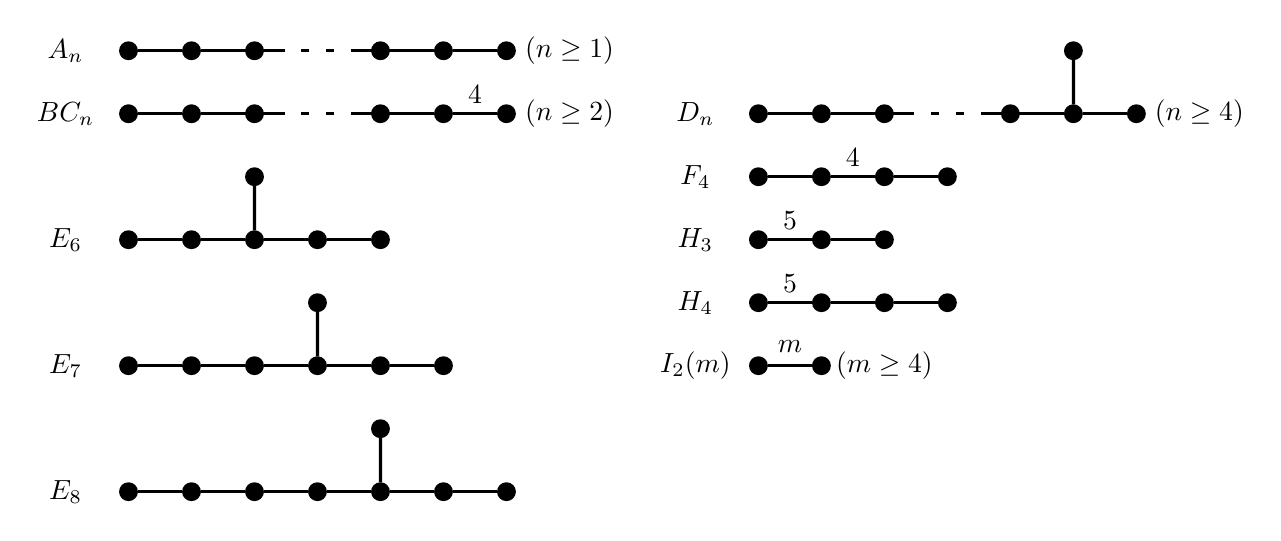
\begin{tikzpicture}[scale = 0.8]
    \begin{scope}[shift={(0,0)}]
        \node at (0,0) {$A_n$};
        \begin{scope}[every node/.style={circle, fill=black, draw, thick, minimum size = 6pt, inner sep=0pt}]
            \node (1) at (1,0) {};
            \node (2) at (2,0) {};
            \node (3) at (3,0) {};
            \node (n-2) at (5,0) {};
            \node (n-1) at (6,0) {};
            \node (n) at (7,0) {};
        \end{scope}
        \node (3a) at (3.5,0) {};
        \node (3b) at (4.5,0) {};
        \begin{scope}[every edge/.style={draw,very thick}]
            \path [-] (1) edge (2);
            \path [-] (2) edge (3a);
            \path [loosely dashed] (3a.west) edge (3b.east);
            \path [-] (3b) edge (n-1);
            \path [-] (n-1) edge (n);
        \end{scope}
        \node at (8,0) {$(n\geq 1)$};
    \end{scope}

    \begin{scope}[shift={(0,-1)}]
        \node at (0,0) {$BC_n$};
        \begin{scope}[every node/.style={circle, fill=black, draw, thick, minimum size = 6pt, inner sep=0pt}]
            \node (1) at (1,0) {};
            \node (2) at (2,0) {};
            \node (3) at (3,0) {};
            \node (n-2) at (5,0) {};
            \node (n-1) at (6,0) {};
            \node (n) at (7,0) {};
        \end{scope}
        \node (3a) at (3.5,0) {};
        \node (3b) at (4.5,0) {};
        \begin{scope}[every edge/.style={draw,very thick}]
            \path [-] (1) edge (2);
            \path [-] (2) edge (3a);
            \path [loosely dashed] (3a.west) edge (3b.east);
            \path [-] (3b) edge (n-1);
            \path [-] (n-1) edge (n);
            \node at (6.5,0.3) {$4$};
        \end{scope}
        \node at (8,0) {$(n\geq 2)$};
    \end{scope}

    \begin{scope}[shift={(10,-1)}]
        \node at (0,0) {$D_n$};
        \begin{scope}[every node/.style={circle, fill=black, draw, thick, minimum size = 6pt, inner sep=0pt}]
            \node (1) at (1,0) {};
            \node (2) at (2,0) {};
            \node (3) at (3,0) {};
            \node (n-2) at (5,0) {};
            \node (n-1) at (6,0) {};
            \node (n-1a) at (6,1) {};
            \node (n) at (7,0) {};
        \end{scope}
        \node (3a) at (3.5,0) {};
        \node (3b) at (4.5,0) {};
        \begin{scope}[every edge/.style={draw,very thick}]
            \path [-] (1) edge (2);
            \path [-] (2) edge (3a);
            \path [loosely dashed] (3a.west) edge (3b.east);
            \path [-] (3b) edge (n-1);
            \path [-] (n-1) edge (n-1a);
            \path [-] (n-1) edge (n);
        \end{scope}
        \node at (8,0) {$(n\geq 4)$};
    \end{scope}

    \begin{scope}[shift={(0,-3)}]
        \node at (0,0) {$E_6$};
        \begin{scope}[every node/.style={circle, fill=black, draw, thick, minimum size = 6pt, inner sep=0pt}]
            \node (1) at (1,0) {};
            \node (2) at (2,0) {};
            \node (3) at (3,0) {};
            \node (4) at (3,1) {};
            \node (5) at (4,0) {};
            \node (6) at (5,0) {};
        \end{scope}
        \begin{scope}[every edge/.style={draw,very thick}]
            \path [-] (1) edge (2);
            \path [-] (2) edge (3);
            \path [-] (3) edge (4);
            \path [-] (3) edge (5);
            \path [-] (5) edge (6);
        \end{scope}
    \end{scope}

    \begin{scope}[shift={(0,-5)}]
        \node at (0,0) {$E_7$};
        \begin{scope}[every node/.style={circle, fill=black, draw, thick, minimum size = 6pt, inner sep=0pt}]
            \node (1) at (1,0) {};
            \node (2) at (2,0) {};
            \node (3) at (3,0) {};
            \node (4) at (4,0) {};
            \node (5) at (4,1) {};
            \node (6) at (5,0) {};
            \node (7) at (6,0) {};
        \end{scope}
        \begin{scope}[every edge/.style={draw,very thick}]
            \path [-] (1) edge (2);
            \path [-] (2) edge (3);
            \path [-] (3) edge (4);
            \path [-] (4) edge (5);
            \path [-] (4) edge (6);
            \path [-] (6) edge (7);
        \end{scope}
    \end{scope}

    \begin{scope}[shift={(0,-7)}]
        \node at (0,0) {$E_8$};
        \begin{scope}[every node/.style={circle, fill=black, draw, thick, minimum size = 6pt, inner sep=0pt}]
            \node (1) at (1,0) {};
            \node (2) at (2,0) {};
            \node (3) at (3,0) {};
            \node (4) at (4,0) {};
            \node (5) at (5,0) {};
            \node (6) at (5,1) {};
            \node (7) at (6,0) {};
            \node (8) at (7,0) {};
        \end{scope}
        \begin{scope}[every edge/.style={draw,very thick}]
            \path [-] (1) edge (2);
            \path [-] (2) edge (3);
            \path [-] (3) edge (4);
            \path [-] (4) edge (5);
            \path [-] (5) edge (6);
            \path [-] (5) edge (7);
            \path [-] (7) edge (8);
        \end{scope}
    \end{scope}

    \begin{scope}[shift={(10,-2)}]
        \node at (0,0) {$F_4$};
        \begin{scope}[every node/.style={circle, fill=black, draw, thick, minimum size = 6pt, inner sep=0pt}]
            \node (1) at (1,0) {};
            \node (2) at (2,0) {};
            \node (3) at (3,0) {};
            \node (4) at (4,0) {};
        \end{scope}
        \begin{scope}[every edge/.style={draw,very thick}]
            \path [-] (1) edge (2);
            \path [-] (2) edge (3);
            \path [-] (3) edge (4);
            \node at (2.5,0.3) {$4$};
        \end{scope}
    \end{scope}

    \begin{scope}[shift={(10,-3)}]
        \node at (0,0) {$H_3$};
        \begin{scope}[every node/.style={circle, fill=black, draw, thick, minimum size = 6pt, inner sep=0pt}]
            \node (1) at (1,0) {};
            \node (2) at (2,0) {};
            \node (3) at (3,0) {};
        \end{scope}
        \begin{scope}[every edge/.style={draw,very thick}]
            \path [-] (1) edge (2);
            \path [-] (2) edge (3);
            \node at (1.5,0.3) {$5$};
        \end{scope}
    \end{scope}

    \begin{scope}[shift={(10,-4)}]
        \node at (0,0) {$H_4$};
        \begin{scope}[every node/.style={circle, fill=black, draw, thick, minimum size = 6pt, inner sep=0pt}]
            \node (1) at (1,0) {};
            \node (2) at (2,0) {};
            \node (3) at (3,0) {};
            \node (4) at (4,0) {};
        \end{scope}
        \begin{scope}[every edge/.style={draw,very thick}]
            \path [-] (1) edge (2);
            \path [-] (2) edge (3);
            \path [-] (3) edge (4);
            \node at (1.5,0.3) {$5$};
        \end{scope}
    \end{scope}

    \begin{scope}[shift={(10,-5)}]
        \node at (0,0) {$I_2(m)$};
        \begin{scope}[every node/.style={circle, fill=black, draw, thick, minimum size = 6pt, inner sep=0pt}]
            \node (1) at (1,0) {};
            \node (2) at (2,0) {};
        \end{scope}
        \begin{scope}[every edge/.style={draw,very thick}]
            \path [-] (1) edge (2);
            \node at (1.5,0.3) {$m$};
            \node at (3,0) {$(m\geq 4)$};
        \end{scope}
    \end{scope}
\end{tikzpicture}
\caption{Positive definite Coxeter diagrams}
\label{fig:posdef}
\end{figure}

And here is another collection who can all be founded to be only positive semidefinite:

\begin{figure}[H]
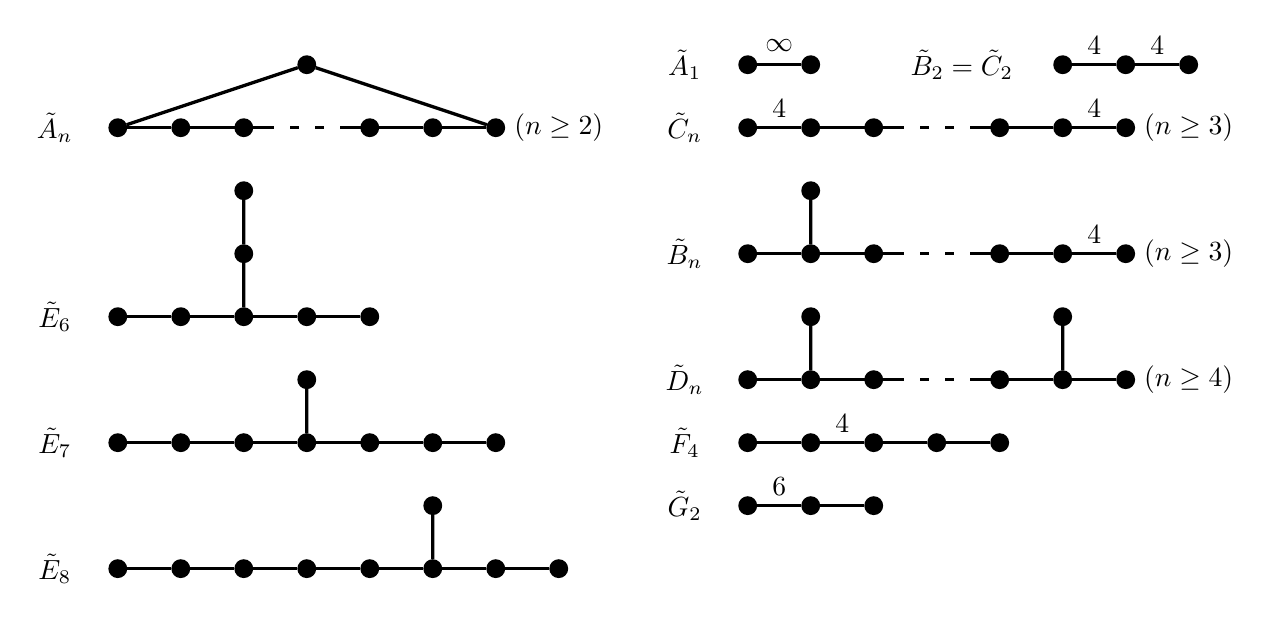
\begin{tikzpicture}[scale = 0.8]
    
    \begin{scope}[shift={(0,0)}] %An
        \node at (0,0) {$\tilde{A}_n$};
        \begin{scope}[every node/.style={circle, fill=black, draw, thick, minimum size = 6pt, inner sep=0pt}]
            \node (1) at (1,0) {};
            \node (2) at (2,0) {};
            \node (3) at (3,0) {};
            \node (n-2) at (5,0) {};
            \node (n-1) at (6,0) {};
            \node (n) at (7,0) {};
            \node (mid) at (4,1) {};
        \end{scope}
        \node (3a) at (3.5,0) {};
        \node (3b) at (4.5,0) {};
        \begin{scope}[every edge/.style={draw,very thick}]
            \path [-] (1) edge (2);
            \path [-] (2) edge (3a);
            \path [loosely dashed] (3a.west) edge (3b.east);
            \path [-] (3b) edge (n-1);
            \path [-] (n-1) edge (n);
            \path [-] (1) edge (mid);
            \path [-] (n) edge (mid);
        \end{scope}
        \node at (8,0) {$(n\geq 2)$};
    \end{scope}

    \begin{scope}[shift={(10,1)}] %A1
        \node at (0,0) {$\tilde{A}_1$};
        \begin{scope}[every node/.style={circle, fill=black, draw, thick, minimum size = 6pt, inner sep=0pt}]
            \node (1) at (1,0) {};
            \node (2) at (2,0) {};
        \end{scope}
        \begin{scope}[every edge/.style={draw,very thick}]
            \path [-] (1) edge (2);
            \node at (1.5,0.3) {$\infty$};
        \end{scope}
    \end{scope}

    \begin{scope}[shift={(15,1)}] %bc2
        \node at (-0.6,0) {$\tilde{B}_2=\tilde{C}_2$};
        \begin{scope}[every node/.style={circle, fill=black, draw, thick, minimum size = 6pt, inner sep=0pt}]
            \node (1) at (1,0) {};
            \node (2) at (2,0) {};
            \node (3) at (3,0) {};
        \end{scope}
        \begin{scope}[every edge/.style={draw,very thick}]
            \path [-] (1) edge (2);
            \path [-] (2) edge (3);
            \node at (1.5,0.3) {$4$};
            \node at (2.5,0.3) {$4$};
        \end{scope}
    \end{scope}

    \begin{scope}[shift={(10,0)}] %cn
        \node at (0,0) {$\tilde{C}_n$};
        \begin{scope}[every node/.style={circle, fill=black, draw, thick, minimum size = 6pt, inner sep=0pt}]
            \node (1) at (1,0) {};
            \node (2) at (2,0) {};
            \node (3) at (3,0) {};
            \node (n-2) at (5,0) {};
            \node (n-1) at (6,0) {};
            \node (n) at (7,0) {};
        \end{scope}
        \node (3a) at (3.5,0) {};
        \node (3b) at (4.5,0) {};
        \begin{scope}[every edge/.style={draw,very thick}]
            \path [-] (1) edge (2);
            \path [-] (2) edge (3a);
            \path [loosely dashed] (3a.west) edge (3b.east);
            \path [-] (3b) edge (n-1);
            \path [-] (n-1) edge (n);
            \node at (6.5,0.3) {$4$};
            \node at (1.5,0.3) {$4$};
        \end{scope}
        \node at (8,0) {$(n\geq 3)$};
    \end{scope}

    \begin{scope}[shift={(10,-2)}] %bn
        \node at (0,0) {$\tilde{B}_n$};
        \begin{scope}[every node/.style={circle, fill=black, draw, thick, minimum size = 6pt, inner sep=0pt}]
            \node (1) at (1,0) {};
            \node (2) at (2,0) {};
            \node (2a) at (2,1) {};
            \node (3) at (3,0) {};
            \node (n-2) at (5,0) {};
            \node (n-1) at (6,0) {};
            \node (n) at (7,0) {};
        \end{scope}
        \node (3a) at (3.5,0) {};
        \node (3b) at (4.5,0) {};
        \begin{scope}[every edge/.style={draw,very thick}]
            \path [-] (1) edge (2);
            \path [-] (2) edge (3a);
            \path [loosely dashed] (3a.west) edge (3b.east);
            \path [-] (3b) edge (n-1);
            \path [-] (2) edge (2a);
            \path [-] (n-1) edge (n);
            \node at (6.5,0.3) {$4$};
        \end{scope}
        \node at (8,0) {$(n\geq 3)$};
    \end{scope}

    \begin{scope}[shift={(10,-4)}] %dn
        \node at (0,0) {$\tilde{D}_n$};
        \begin{scope}[every node/.style={circle, fill=black, draw, thick, minimum size = 6pt, inner sep=0pt}]
            \node (1) at (1,0) {};
            \node (2) at (2,0) {};
            \node (2a) at (2,1) {};
            \node (3) at (3,0) {};
            \node (n-2) at (5,0) {};
            \node (n-1) at (6,0) {};
            \node (n-1a) at (6,1) {};
            \node (n) at (7,0) {};
        \end{scope}
        \node (3a) at (3.5,0) {};
        \node (3b) at (4.5,0) {};
        \begin{scope}[every edge/.style={draw,very thick}]
            \path [-] (1) edge (2);
            \path [-] (2) edge (2a);
            \path [-] (2) edge (3a);
            \path [loosely dashed] (3a.west) edge (3b.east);
            \path [-] (3b) edge (n-1);
            \path [-] (n-1) edge (n-1a);
            \path [-] (n-1) edge (n);
        \end{scope}
        \node at (8,0) {$(n\geq 4)$};
    \end{scope}

    \begin{scope}[shift={(0,-3)}] %e6
        \node at (0,0) {$\tilde{E}_6$};
        \begin{scope}[every node/.style={circle, fill=black, draw, thick, minimum size = 6pt, inner sep=0pt}]
            \node (1) at (1,0) {};
            \node (2) at (2,0) {};
            \node (3) at (3,0) {};
            \node (3a) at (3,1) {};
            \node (3b) at (3,2) {};
            \node (4) at (4,0) {};
            \node (5) at (5,0) {};
        \end{scope}
        \begin{scope}[every edge/.style={draw,very thick}]
            \path [-] (1) edge (2);
            \path [-] (2) edge (3);
            \path [-] (3) edge (3a);
            \path [-] (3a) edge (3b);
            \path [-] (3) edge (4);
            \path [-] (4) edge (5);
        \end{scope}
    \end{scope}

    \begin{scope}[shift={(0,-5)}] %e7
        \node at (0,0) {$\tilde{E}_7$};
        \begin{scope}[every node/.style={circle, fill=black, draw, thick, minimum size = 6pt, inner sep=0pt}]
            \node (1) at (1,0) {};
            \node (2) at (2,0) {};
            \node (3) at (3,0) {};
            \node (4) at (4,0) {};
            \node (4a) at (4,1) {};
            \node (5) at (5,0) {};
            \node (6) at (6,0) {};
            \node (7) at (7,0) {};
        \end{scope}
        \begin{scope}[every edge/.style={draw,very thick}]
            \path [-] (1) edge (2);
            \path [-] (2) edge (3);
            \path [-] (3) edge (4);
            \path [-] (4) edge (4a);
            \path [-] (4) edge (5);
            \path [-] (4) edge (6);
            \path [-] (6) edge (7);
        \end{scope}
    \end{scope}

    \begin{scope}[shift={(0,-7)}] %e8
        \node at (0,0) {$\tilde{E}_8$};
        \begin{scope}[every node/.style={circle, fill=black, draw, thick, minimum size = 6pt, inner sep=0pt}]
            \node (1) at (1,0) {};
            \node (2) at (2,0) {};
            \node (3) at (3,0) {};
            \node (4) at (4,0) {};
            \node (5) at (5,0) {};
            \node (6) at (6,0) {};
            \node (6a) at (6,1) {};
            \node (7) at (7,0) {};
            \node (8) at (8,0) {};
        \end{scope}
        \begin{scope}[every edge/.style={draw,very thick}]
            \path [-] (1) edge (2);
            \path [-] (2) edge (3);
            \path [-] (3) edge (4);
            \path [-] (4) edge (5);
            \path [-] (5) edge (6);
            \path [-] (6) edge (7);
            \path [-] (6) edge (6a);
            \path [-] (7) edge (8);
        \end{scope}
    \end{scope}

    \begin{scope}[shift={(10,-5)}] %f4
        \node at (0,0) {$\tilde{F}_4$};
        \begin{scope}[every node/.style={circle, fill=black, draw, thick, minimum size = 6pt, inner sep=0pt}]
            \node (1) at (1,0) {};
            \node (2) at (2,0) {};
            \node (3) at (3,0) {};
            \node (4) at (4,0) {};
            \node (5) at (5,0) {};
        \end{scope}
        \begin{scope}[every edge/.style={draw,very thick}]
            \path [-] (1) edge (2);
            \path [-] (2) edge (3);
            \path [-] (3) edge (4);
            \path [-] (4) edge (5);
            \node at (2.5,0.3) {$4$};
        \end{scope}
    \end{scope}

    \begin{scope}[shift={(10,-6)}] %g2
        \node at (0,0) {$\tilde{G}_2$};
        \begin{scope}[every node/.style={circle, fill=black, draw, thick, minimum size = 6pt, inner sep=0pt}]
            \node (1) at (1,0) {};
            \node (2) at (2,0) {};
            \node (3) at (3,0) {};
        \end{scope}
        \begin{scope}[every edge/.style={draw,very thick}]
            \path [-] (1) edge (2);
            \path [-] (2) edge (3);
            \node at (1.5,0.3) {$6$};
        \end{scope}
    \end{scope}

\end{tikzpicture}
\caption{Positive semidefinite Coxeter diagrams}
\label{fig:possemidef}
\end{figure}

Plus two helper diagrams which are neither:

\begin{figure}[H]
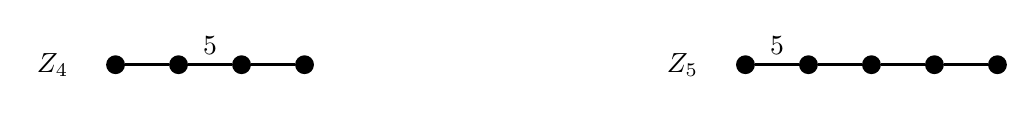
\begin{tikzpicture}[scale = 0.8]

    \begin{scope}[shift={(0,0)}] %A1
        \node at (0,0) {$Z_4$};
        \begin{scope}[every node/.style={circle, fill=black, draw, thick, minimum size = 6pt, inner sep=0pt}]
            \node (1) at (1,0) {};
            \node (2) at (2,0) {};
            \node (3) at (3,0) {};
            \node (4) at (4,0) {};
        \end{scope}
        \begin{scope}[every edge/.style={draw,very thick}]
            \path [-] (1) edge (2);
            \path [-] (2) edge (3);
            \path [-] (3) edge (4);
            \node at (2.5,0.3) {$5$};
        \end{scope}
    \end{scope}

    \begin{scope}[shift={(10,0)}] %A1
        \node at (0,0) {$Z_5$};
        \begin{scope}[every node/.style={circle, fill=black, draw, thick, minimum size = 6pt, inner sep=0pt}]
            \node (1) at (1,0) {};
            \node (2) at (2,0) {};
            \node (3) at (3,0) {};
            \node (4) at (4,0) {};
            \node (5) at (5,0) {};
        \end{scope}
        \begin{scope}[every edge/.style={draw,very thick}]
            \path [-] (1) edge (2);
            \path [-] (2) edge (3);
            \path [-] (3) edge (4);
            \path [-] (4) edge (5);
            \node at (1.5,0.3) {$5$};
        \end{scope}
    \end{scope}

\end{tikzpicture}
\caption{Helper Coxeter diagrams}
\label{fig:helper}
\end{figure}

\begin{theorem}
    the diagrams of Figure \ref{fig:posdef} are all the connected diagrams with positive definite quadratic form.
    \begin{proof}
        The proof goes by indentifying features present in the graphs of Figure \ref{fig:possemidef}, observing they cannot appear as subdiagrams of those with positive definite quadratic form: e.g. no cycles as in $\tilde{A}_n$ and all edges must be finite due to $\tilde{A}_1$. For the full proof see \cite{Humphreys1990}.
    \end{proof}
\end{theorem}

\begin{corollary}
    The following graphs categorise all finite reflection groups.
    \begin{proof}
        We know it suffices to classify the reflections groups corresponding to connected Coxeter diagrams, all of which must have positive definited associated quadratic form, all of which we have found. The only remaining step is to find polytopes admitting these Coxeter groups as their reflection groups, lots of these examples have been seen in the previous section, and in fact every diagram of Figure \ref{fig:posdef} does occur as a finite reflection.
    \end{proof}
\end{corollary}

This solution can seem somewhat unsatisfactory as there is no immediate reason as to \textbf{why} all of the finite Coxeter groups can be realised as reflection groups.

\subsection{Geometric representation}\label{geom:rep}

For any finite Coxeter system $(W,S)$ consider the abstract real vector space $V$ with basis $\Phi$. We can define a quadratic form (and thus an inner product  $\abr{-,-}$) on $V$ in the same way as we did earlier. And for each generator $s\in S$ we can associate a reflection $\sigma_s:V\rightarrow V$ given natrually as $\sigma_s (v) = v-2\abr{\alpha_s,v}\alpha_s$. Through some similar calculations we can find the representation this induces on $W$ is faithful and acts orthogonally on $V$, the construction of the edges and vertices of a polytope demonstrated in the next section will thus show how a regular polytope can be realised from this abstract reflection group.

% \begin{figure}[H]
% \resizebox{\textwidth}{!}{
% \begin{tikzpicture}
%     \begin{scope}[shift={(0,0)}]
%         \node at (0,0) {$A_n$};
%         \begin{scope}[every node/.style={circle, fill=black, draw, thick, minimum size = 6pt, inner sep=0pt}]
%             \node (1) at (2,0) {};
%             \node (2) at (4,0) {};
%             \node (3) at (6,0) {};
%             \node (n-2) at (10,0) {};
%             \node (n-1) at (12,0) {};
%             \node (n) at (14,0) {};
%         \end{scope}
%         \node (3a) at (7,0) {};
%         \node (3b) at (9,0) {};
%         \begin{scope}[every edge/.style={draw,very thick}]
%             \path [-] (1) edge (2);
%             \path [-] (2) edge (3a);
%             \path [loosely dashed] (3a.west) edge (3b.east);
%             \path [-] (3b) edge (n-1);
%             \path [-] (n-1) edge (n);
%         \end{scope}
%         \node at (16,0) {$(n\geq 1)$};
%     \end{scope}

%     \begin{scope}[shift={(0,-1.5)}]
%         \node at (0,0) {$BC_n$};
%         \begin{scope}[every node/.style={circle, fill=black, draw, thick, minimum size = 6pt, inner sep=0pt}]
%             \node (1) at (2,0) {};
%             \node (2) at (4,0) {};
%             \node (3) at (6,0) {};
%             \node (n-2) at (10,0) {};
%             \node (n-1) at (12,0) {};
%             \node (n) at (14,0) {};
%         \end{scope}
%         \node (3a) at (7,0) {};
%         \node (3b) at (9,0) {};
%         \begin{scope}[every edge/.style={draw,very thick}]
%             \path [-] (1) edge (2);
%             \path [-] (2) edge (3a);
%             \path [loosely dashed] (3a.west) edge (3b.east);
%             \path [-] (3b) edge (n-1);
%             \path [-] (n-1) edge (n);
%             \node at (13,0.3) {$4$};
%         \end{scope}
%         \node at (16,0) {$(n\geq 2)$};
%     \end{scope}

%     \begin{scope}[shift={(0,-5)}]
%         \node at (0,0) {$D_n$};
%         \begin{scope}[every node/.style={circle, fill=black, draw, thick, minimum size = 6pt, inner sep=0pt}]
%             \node (1) at (2,0) {};
%             \node (2) at (4,0) {};
%             \node (3) at (6,0) {};
%             \node (n-2) at (10,0) {};
%             \node (n-1) at (12,0) {};
%             \node (n-1a) at (12,2) {};
%             \node (n) at (14,0) {};
%         \end{scope}
%         \node (3a) at (7,0) {};
%         \node (3b) at (9,0) {};
%         \begin{scope}[every edge/.style={draw,very thick}]
%             \path [-] (1) edge (2);
%             \path [-] (2) edge (3a);
%             \path [loosely dashed] (3a.west) edge (3b.east);
%             \path [-] (3b) edge (n-1);
%             \path [-] (n-1) edge (n-1a);
%             \path [-] (n-1) edge (n);
%         \end{scope}
%         \node at (16,0) {$(n\geq 4)$};
%     \end{scope}

%     \begin{scope}[shift={(0,-8.5)}]
%         \node at (0,0) {$E_6$};
%         \begin{scope}[every node/.style={circle, fill=black, draw, thick, minimum size = 6pt, inner sep=0pt}]
%             \node (1) at (2,0) {};
%             \node (2) at (4,0) {};
%             \node (3) at (6,0) {};
%             \node (4) at (6,2) {};
%             \node (5) at (8,0) {};
%             \node (6) at (10,0) {};
%         \end{scope}
%         \begin{scope}[every edge/.style={draw,very thick}]
%             \path [-] (1) edge (2);
%             \path [-] (2) edge (3);
%             \path [-] (3) edge (4);
%             \path [-] (3) edge (5);
%             \path [-] (5) edge (6);
%         \end{scope}
%     \end{scope}

%     \begin{scope}[shift={(0,-12)}]
%         \node at (0,0) {$E_7$};
%         \begin{scope}[every node/.style={circle, fill=black, draw, thick, minimum size = 6pt, inner sep=0pt}]
%             \node (1) at (2,0) {};
%             \node (2) at (4,0) {};
%             \node (3) at (6,0) {};
%             \node (4) at (8,0) {};
%             \node (5) at (8,2) {};
%             \node (6) at (10,0) {};
%             \node (7) at (12,0) {};
%         \end{scope}
%         \begin{scope}[every edge/.style={draw,very thick}]
%             \path [-] (1) edge (2);
%             \path [-] (2) edge (3);
%             \path [-] (3) edge (4);
%             \path [-] (4) edge (5);
%             \path [-] (4) edge (6);
%             \path [-] (6) edge (7);
%         \end{scope}
%     \end{scope}

%     \begin{scope}[shift={(0,-15.5)}]
%         \node at (0,0) {$E_8$};
%         \begin{scope}[every node/.style={circle, fill=black, draw, thick, minimum size = 6pt, inner sep=0pt}]
%             \node (1) at (2,0) {};
%             \node (2) at (4,0) {};
%             \node (3) at (6,0) {};
%             \node (4) at (8,0) {};
%             \node (5) at (10,0) {};
%             \node (6) at (10,2) {};
%             \node (7) at (12,0) {};
%             \node (8) at (14,0) {};
%         \end{scope}
%         \begin{scope}[every edge/.style={draw,very thick}]
%             \path [-] (1) edge (2);
%             \path [-] (2) edge (3);
%             \path [-] (3) edge (4);
%             \path [-] (4) edge (5);
%             \path [-] (5) edge (6);
%             \path [-] (5) edge (7);
%             \path [-] (7) edge (8);
%         \end{scope}
%     \end{scope}

%     \begin{scope}[shift={(0,-17)}]
%         \node at (0,0) {$F_4$};
%         \begin{scope}[every node/.style={circle, fill=black, draw, thick, minimum size = 6pt, inner sep=0pt}]
%             \node (1) at (2,0) {};
%             \node (2) at (4,0) {};
%             \node (3) at (6,0) {};
%             \node (4) at (8,0) {};
%         \end{scope}
%         \begin{scope}[every edge/.style={draw,very thick}]
%             \path [-] (1) edge (2);
%             \path [-] (2) edge (3);
%             \path [-] (3) edge (4);
%             \node at (5,0.3) {$4$};
%         \end{scope}
%     \end{scope}

%     \begin{scope}[shift={(0,-18.5)}]
%         \node at (0,0) {$H_3$};
%         \begin{scope}[every node/.style={circle, fill=black, draw, thick, minimum size = 6pt, inner sep=0pt}]
%             \node (1) at (2,0) {};
%             \node (2) at (4,0) {};
%             \node (3) at (6,0) {};
%         \end{scope}
%         \begin{scope}[every edge/.style={draw,very thick}]
%             \path [-] (1) edge (2);
%             \path [-] (2) edge (3);
%             \node at (3,0.3) {$5$};
%         \end{scope}
%     \end{scope}

%     \begin{scope}[shift={(0,-20)}]
%         \node at (0,0) {$H_4$};
%         \begin{scope}[every node/.style={circle, fill=black, draw, thick, minimum size = 6pt, inner sep=0pt}]
%             \node (1) at (2,0) {};
%             \node (2) at (4,0) {};
%             \node (3) at (6,0) {};
%             \node (4) at (8,0) {};
%         \end{scope}
%         \begin{scope}[every edge/.style={draw,very thick}]
%             \path [-] (1) edge (2);
%             \path [-] (2) edge (3);
%             \path [-] (3) edge (4);
%             \node at (3,0.3) {$5$};
%         \end{scope}
%     \end{scope}

%     \begin{scope}[shift={(0,-21.5)}]
%         \node at (0,0) {$I_2(m)$};
%         \begin{scope}[every node/.style={circle, fill=black, draw, thick, minimum size = 6pt, inner sep=0pt}]
%             \node (1) at (2,0) {};
%             \node (2) at (4,0) {};
%         \end{scope}
%         \begin{scope}[every edge/.style={draw,very thick}]
%             \path [-] (1) edge (2);
%             \node at (3,0.3) {$m$};
%             \node at (6,0) {$(m\geq 4)$};
%         \end{scope}
%     \end{scope}
% \end{tikzpicture}
% }
% \end{figure}


\end{document}